\documentclass[a4paper,12pt]{article}
\usepackage[utf8]{inputenc}
\usepackage[T2A]{fontenc}
\usepackage[russian]{babel}
\usepackage{amsmath, amssymb, amsfonts, amsthm}
\usepackage{graphicx}
\usepackage{geometry}
\usepackage{float}
\usepackage[hidelinks, pdfencoding=auto, psdextra]{hyperref}
\usepackage{tocloft}
\usepackage{fancyhdr}
\usepackage{enumitem}
\usepackage{listings}
\usepackage{xcolor}
\usepackage{subcaption}

\geometry{top=2cm, bottom=2cm, left=2.5cm, right=2cm}
\setlength{\headheight}{14.5pt}

\begin{document}

\begin{titlepage}
    \centering
    {\Large \bfseries Федеральное государственное автономное образовательное учреждение высшего образования «Национальный исследовательский университет ИТМО» \par}
    
    {\large Факультет программной инженерии и компьютерной техники \par}
    \vspace{2cm}
    {\LARGE Домашнее задание №1 \par}
    \vspace{0.5cm}
    {\Large Вариант 74 \par}
    \vspace{2cm}
    \vfill
    \begin{flushright}
        \large
        \textbf{Выполнил:} \\
        Шулай Роман \\
        Группа P3115 \\
        \vspace{1cm}
        \textbf{Преподаватель:} \\
        Поляков Владимир Иванович \\
    \end{flushright}
    \vfill
    {\large Санкт-Петербург \\ 2026 год}
\end{titlepage}
\newpage
\setcounter{page}{2}

\begin{figure}[htbp]
    \centering
    \begin{subfigure}[b]{0.45\textwidth}
        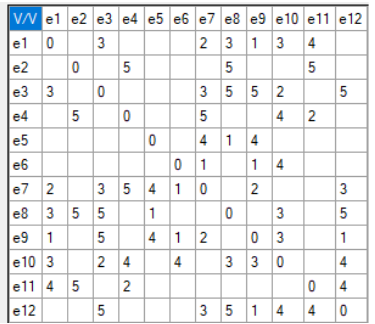
\includegraphics[width=\linewidth]{images/matrix.png}
        \caption{Матрица смежности}
        \label{fig:sub1}
    \end{subfigure}
    \hfill % Распорка для равномерного распределения
    \begin{subfigure}[b]{0.45\textwidth}
        
\includegraphics[width=\linewidth]{images/graph.png}
        \caption{Граф}
        \label{fig:sub2}
    \end{subfigure}
    %\caption{Общая подпись для двух картинок}
    \label{fig:main}
\end{figure}

\begin{table}[H]
    \centering
    \begin{tabular}{|l|l|l|l|l|l|l|l|l|l|l|l|l|l|}
    \hline
        v/v & $e_1$ & $e_2$ & $e_3$ & $e_4$ & $e_5$ & $e_6$ & $e_7$ & $e_8$ & $e_9$ & $e_{10}$ & $e_{11}$ & $e_{12}$ & $r_i$ \\ \hline
        $e_1$ & 0 & 0 & 1 & 0 & 0 & 0 & 1 & 1 & 1 & 1 & 1 & 0 & 6 \\ \hline
        $e_2$ & 0 & 0 & 0 & 1 & 0 & 0 & 0 & 1 & 0 & 0 & 1 & 0 & 3 \\ \hline
        $e_3$ & 1 & 0 & 0 & 0 & 0 & 0 & 1 & 1 & 1 & 1 & 0 & 1 & 6 \\ \hline
        $e_4$ & 0 & 1 & 0 & 0 & 0 & 0 & 1 & 0 & 0 & 1 & 1 & 0 & 4 \\ \hline
        $e_5$ & 0 & 0 & 0 & 0 & 0 & 0 & 1 & 1 & 1 & 0 & 0 & 0 & 3 \\ \hline
        $e_6$ & 0 & 0 & 0 & 0 & 0 & 0 & 1 & 0 & 1 & 1 & 0 & 0 & 3 \\ \hline
        $e_7$ & 1 & 0 & 1 & 1 & 1 & 1 & 0 & 0 & 1 & 0 & 0 & 1 & 7 \\ \hline
        $e_8$ & 1 & 1 & 1 & 0 & 1 & 0 & 0 & 0 & 0 & 1 & 0 & 1 & 6 \\ \hline
        $e_9$ & 1 & 0 & 1 & 0 & 1 & 1 & 1 & 0 & 0 & 1 & 0 & 1 & 7 \\ \hline
        $e_{10}$ & 1 & 0 & 1 & 1 & 0 & 1 & 0 & 1 & 1 & 0 & 0 & 1 & 7 \\ \hline
        $e_{11}$ & 1 & 1 & 0 & 1 & 0 & 0 & 0 & 0 & 0 & 0 & 0 & 1 & 4 \\ \hline
        $e_{12}$ & 0 & 0 & 1 & 0 & 0 & 0 & 1 & 1 & 1 & 1 & 1 & 0 & 6 \\ \hline
    \end{tabular}
\end{table}
\noindent 1. Положим $j = 1$ \\
2. Упорядочим вершины в порядке невозрастания $r_i$ \\
$e_7$, $e_9$, $e_{10}$, $e_1$, $e_3$, $e_8$, $e_{12}$, $e_4$, $e_{11}$, $e_2$, $e_5$, $e_6$ \\
3. Красим вершины $e_7$, $e_{10}$, $e_{11}$ в цвет (1) \\
4. Удаляем раскрашенные вершины и переходим к следующему шагу \\
5. $j = j + 1 = 2$ \\
\begin{table}[H]
    \centering
    \begin{tabular}{|l|l|l|l|l|l|l|l|l|l|l|}
    \hline
        v/v & $e_1$ & $e_2$ & $e_3$ & $e_4$ & $e_5$ & $e_6$ & $e_8$ & $e_9$ & $e_{12}$ & $r_i$ \\ \hline
        $e_1$ & 0 & 0 & 1 & 0 & 0 & 0 & 1 & 1 & 0 & 3 \\ \hline
        $e_2$ & 0 & 0 & 0 & 1 & 0 & 0 & 1 & 0 & 0 & 2 \\ \hline
        $e_3$ & 1 & 0 & 0 & 0 & 0 & 0 & 1 & 1 & 1 & 4 \\ \hline
        $e_4$ & 0 & 1 & 0 & 0 & 0 & 0 & 0 & 0 & 0 & 1 \\ \hline
        $e_5$ & 0 & 0 & 0 & 0 & 0 & 0 & 1 & 1 & 0 & 2 \\ \hline
        $e_6$ & 0 & 0 & 0 & 0 & 0 & 0 & 0 & 1 & 0 & 1 \\ \hline
        $e_8$ & 1 & 1 & 1 & 0 & 1 & 0 & 0 & 0 & 1 & 5 \\ \hline
        $e_9$ & 1 & 0 & 1 & 0 & 1 & 1 & 0 & 0 & 1 & 5 \\ \hline
        $e_{12}$ & 0 & 0 & 1 & 0 & 0 & 0 & 1 & 1 & 0 & 3 \\ \hline
    \end{tabular}
\end{table}
\noindent 6. Упорядочим вершины в порядке невозрастания $r_i$ \\
$e_8$, $e_9$, $e_3$, $e_1$, $e_{12}$, $e_2$, $e_5$, $e_4$, $e_6$ \\
7. Красим вершины $e_8$, $e_9$, $e_4$ в цвет (2) \\
8. Удаляем эти вершины и переходим к следующему шагу \\
9. $j = j + 1 = 3$ \\
\begin{table}[H]
    \centering
    \begin{tabular}{|l|l|l|l|l|l|l|l|}
    \hline
        v/v & $e_1$ & $e_2$ & $e_3$ & $e_5$ & $e_6$ & $e_{12}$ & $r_i$ \\ \hline
        $e_1$ & 0 & 0 & 1 & 0 & 0 & 0 & 1 \\ \hline
        $e_2$ & 0 & 0 & 0 & 0 & 0 & 0 & 0 \\ \hline
        $e_3$ & 1 & 0 & 0 & 0 & 0 & 1 & 2 \\ \hline
        $e_5$ & 0 & 0 & 0 & 0 & 0 & 0 & 0 \\ \hline
        $e_6$ & 0 & 0 & 0 & 0 & 0 & 0 & 0 \\ \hline
        $e_{12}$ & 0 & 0 & 1 & 0 & 0 & 0 & 1 \\ \hline
    \end{tabular}
\end{table}
\noindent 10. Упорядочим вершины в порядке невозрастания $r_i$ \\
$e_3$, $e_1$, $e_{12}$, $e_2$, $e_5$, $e_6$ \\
11. Красим вершины $e_3$, $e_2$, $e_5$, $e_6$ в цвет (3) \\
12. Удаляем эти вершины и переходим к следующему шагу \\
13. $j = j + 1 = 4$ \\
\begin{table}[H]
    \centering
    \begin{tabular}{|l|l|l|l|}
    \hline
        v/v & $e_1$ & $e_{12}$ & $r_i$ \\ \hline
        $e_1$ & 0 & 0 & 0 \\ \hline
        $e_{12}$ & 0 & 0 & 0 \\ \hline
    \end{tabular}
\end{table}
\noindent 14. Оставшиеся вершины $e_1$ и $e_{12}$ красим в цвет (4) \\
Итого потребовалось 4 цвета
\begin{figure}[H]
    \centering
    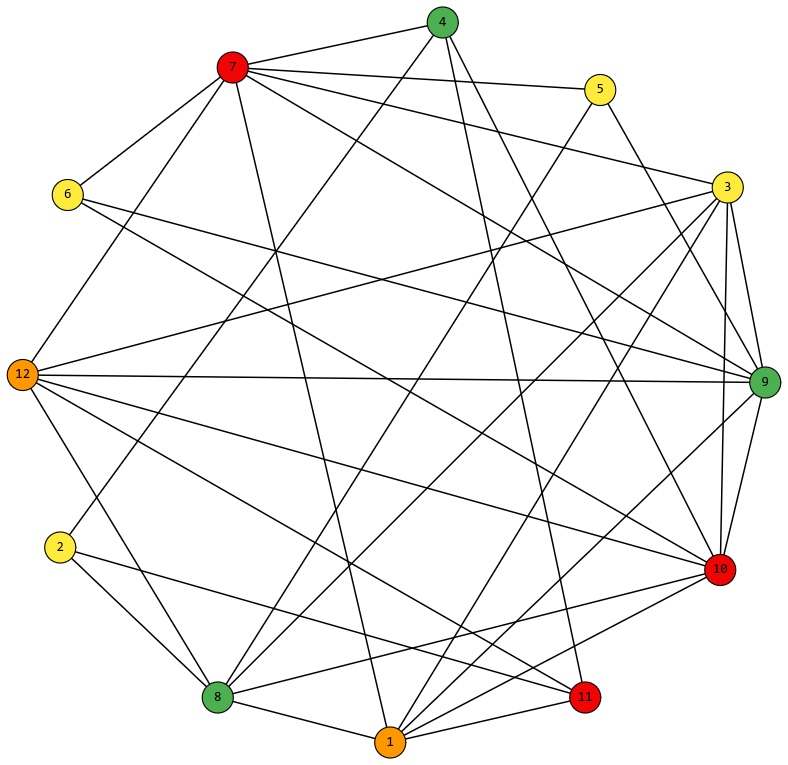
\includegraphics[width=0.5\linewidth]{images/colored.png}
    \caption*{Раскрашенный граф}
\end{figure}

\end{document}
